Using SIMD types

We need to use the SIMD intrinsics of Sunway TaihuLight to make use of its full computing potential.
The SIMD intrinsic expressions accept SIMD types such as
\verb`intv8`,
\verb`doublev4`,
\verb`floatv4`.

In order to convert between scalar types and SIMD types, for example
\verb`double` $\to$ \verb`doublev4`, you may use the dedicated intrinsic functions such as
 \verb`simd_load`,  \verb`simd_loadu`.
You can also
convert between scalar types and SIMD types by
simply pointing \verb`double *` and  \verb`doublev4 *` to the same address. This works just fine.

We can express
computations of
SIMD type variables either by the overloaded arithmetic operators, or by using SIMD intrinsic functions such as
\verb`simd_vmad`.
\begin{center}
  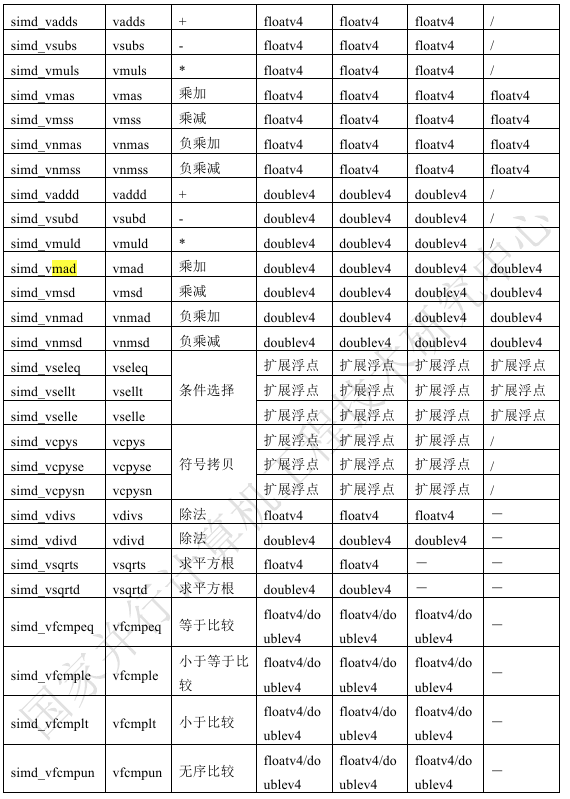
\includegraphics[width=12cm]{figure/sunway-simd.png}
  \end{center}
%%%%


We heve rewritten the previous example using
SIMD types and SIMD operations.
